\documentclass[12pt]{article}    % Add "draft" option for draft mode
\usepackage[paper=a4paper, top=30mm, bottom=30mm]{geometry}

% Font and encoding
\usepackage{lmodern}           % Better computer modern font
\usepackage[T1]{fontenc}       % Better glyph encoding
\usepackage[utf8]{inputenc}    % Necessary for unicode characters
\usepackage[english]{babel}    % Necessary for correct hyphenation
\usepackage{textcomp}          % Necessary to display unicode characters like €
\usepackage{csquotes}          % Quotes (\MakeOuterQuote{"} needed!)

% Other packages
\usepackage[style=authoryear]{biblatex}    % Bibliography
\usepackage[parfill]{parskip}              % Add space between paragraphs
\usepackage[hidelinks]{hyperref}           % Clickable \ref and \cite
\usepackage{graphicx}                      % Needed for figures
\usepackage{booktabs}                      % Needed for tables
\usepackage{caption}                       % Needed for captionsetup
\usepackage{subcaption}                    % Needed for subfigure and subtable
\usepackage{amsmath}                       % Better math environments and \text
\usepackage{physics}                       % e.g. for derivative formatting
\usepackage{siunitx}                       % \si{\unit} and \SI{value}{\unit}
\usepackage{titlesec}                      % Needed for titleformat
\usepackage{authblk}                       % Authors formatting

% Setup
\MakeOuterQuote{"}
% \setcounter{secnumdepth}{0}
% \titleformat{\chapter}{\normalfont\bfseries\Huge}{\thechapter}{20pt}{}
% \setlength{\parskip}{.5\baselineskip}
\setlength\parindent{0pt}
\captionsetup{width=.9\linewidth}
% \captionsetup[subfigure]{width=.9\linewidth}
\addbibresource{bib.bib}

\title{Effects of Layer Freezing when Transferring DeepSpeech from English to German}
\author[1]{\textbf{Onno Eberhard}}
\author[ ]{\textbf{Torsten Zesch}}
\affil[ ]{Language Technology Lab}
\affil[ ]{University of Duisburg-Essen}
\affil[1]{\href{mailto:onno.eberhard@stud.uni-due.de}{\texttt{onno.eberhard@stud.uni-due.de}}}
\date{}

\begin{document}
\maketitle

\begin{abstract}\noindent
In this paper, we train Mozilla's DeepSpeech architecture in various ways on Mozilla's Common Voice German language speech dataset and compare the results. We build on previous efforts by \textcite{agarwal-zesch-2019-german} and reproduce their results by training the model from scratch. We improve upon these results by using an English pretrained version of DeepSpeech for weight initialization and experiment with the effects of freezing different layers during training.
\end{abstract}

\section{Introduction}
The field of automatic speech recognition is dominated by research specific to English. There exist plenty available text-to-speech models pretrained on (and optimized for) the English language. When it comes to German, the range of available pretrained models becomes much sparser. In this paper, we train Mozilla's implementation\footnote{\url{https://github.com/mozilla/DeepSpeech}} of Baidu's DeepSpeech architecture \parencite{hannun2014deep} on German speech data. We use transfer learning to leverage the availability of a pretrained English version of DeepSpeech and observe the difference made by freezing different layers during training. The rationale for using transfer learning is not only that English and German are closely related languages. In fact, one could argue that they are very different in this context, because DeepSpeech is trained to directly infer written characters from audio data and English and German pronunciations of some characters differ greatly. However, the first few layers of the DeepSpeech network are likely not infering the final output character, but rather lower lever features of the spoken input, such as phonemes, which are shared across different languages. Thus this approach should also work for languages which are not related at all. It is to be expected that the model should give better results when trained on a small dataset than a model trained from scratch, because it does not have to learn these lower level features again.

\section{Training}
\subsection{DeepSpeech architecture}
Mozilla's DeepSpeech implementation differs in many ways from the original model presented in \parencite{hannun2014deep}. The architecture is described in detail in the official documentation\footnote{\url{https://deepspeech.readthedocs.io/en/latest/DeepSpeech.html}} and is depicted in Figure \ref{fig:ds}. From the raw speech data, Mel-Frequency Cepstral Coefficients \parencite{imai1983cepstral} are extracted and passed to a 6-layer deep recurrent neural network. The first three layers are fully connected with a ReLU activation function. The fourth layer is a Long Short-Term Memory unit \parencite{hochreiter1997long}. The fifth layer is again fully connected and ReLU activated. The last layer outputs probabilites for each character in the language's alphabet. It is fully connected and uses a softmax activation for normalization. The character-probabilites are used to calculate a Connectionist Temporal Classification (CTC) loss function \parencite{graves2006connectionist}. The weights of the model are optimized using the Adam method \parencite{kingma2014adam} with respect to the CTC loss.

\begin{figure}[ht]
    \centering
    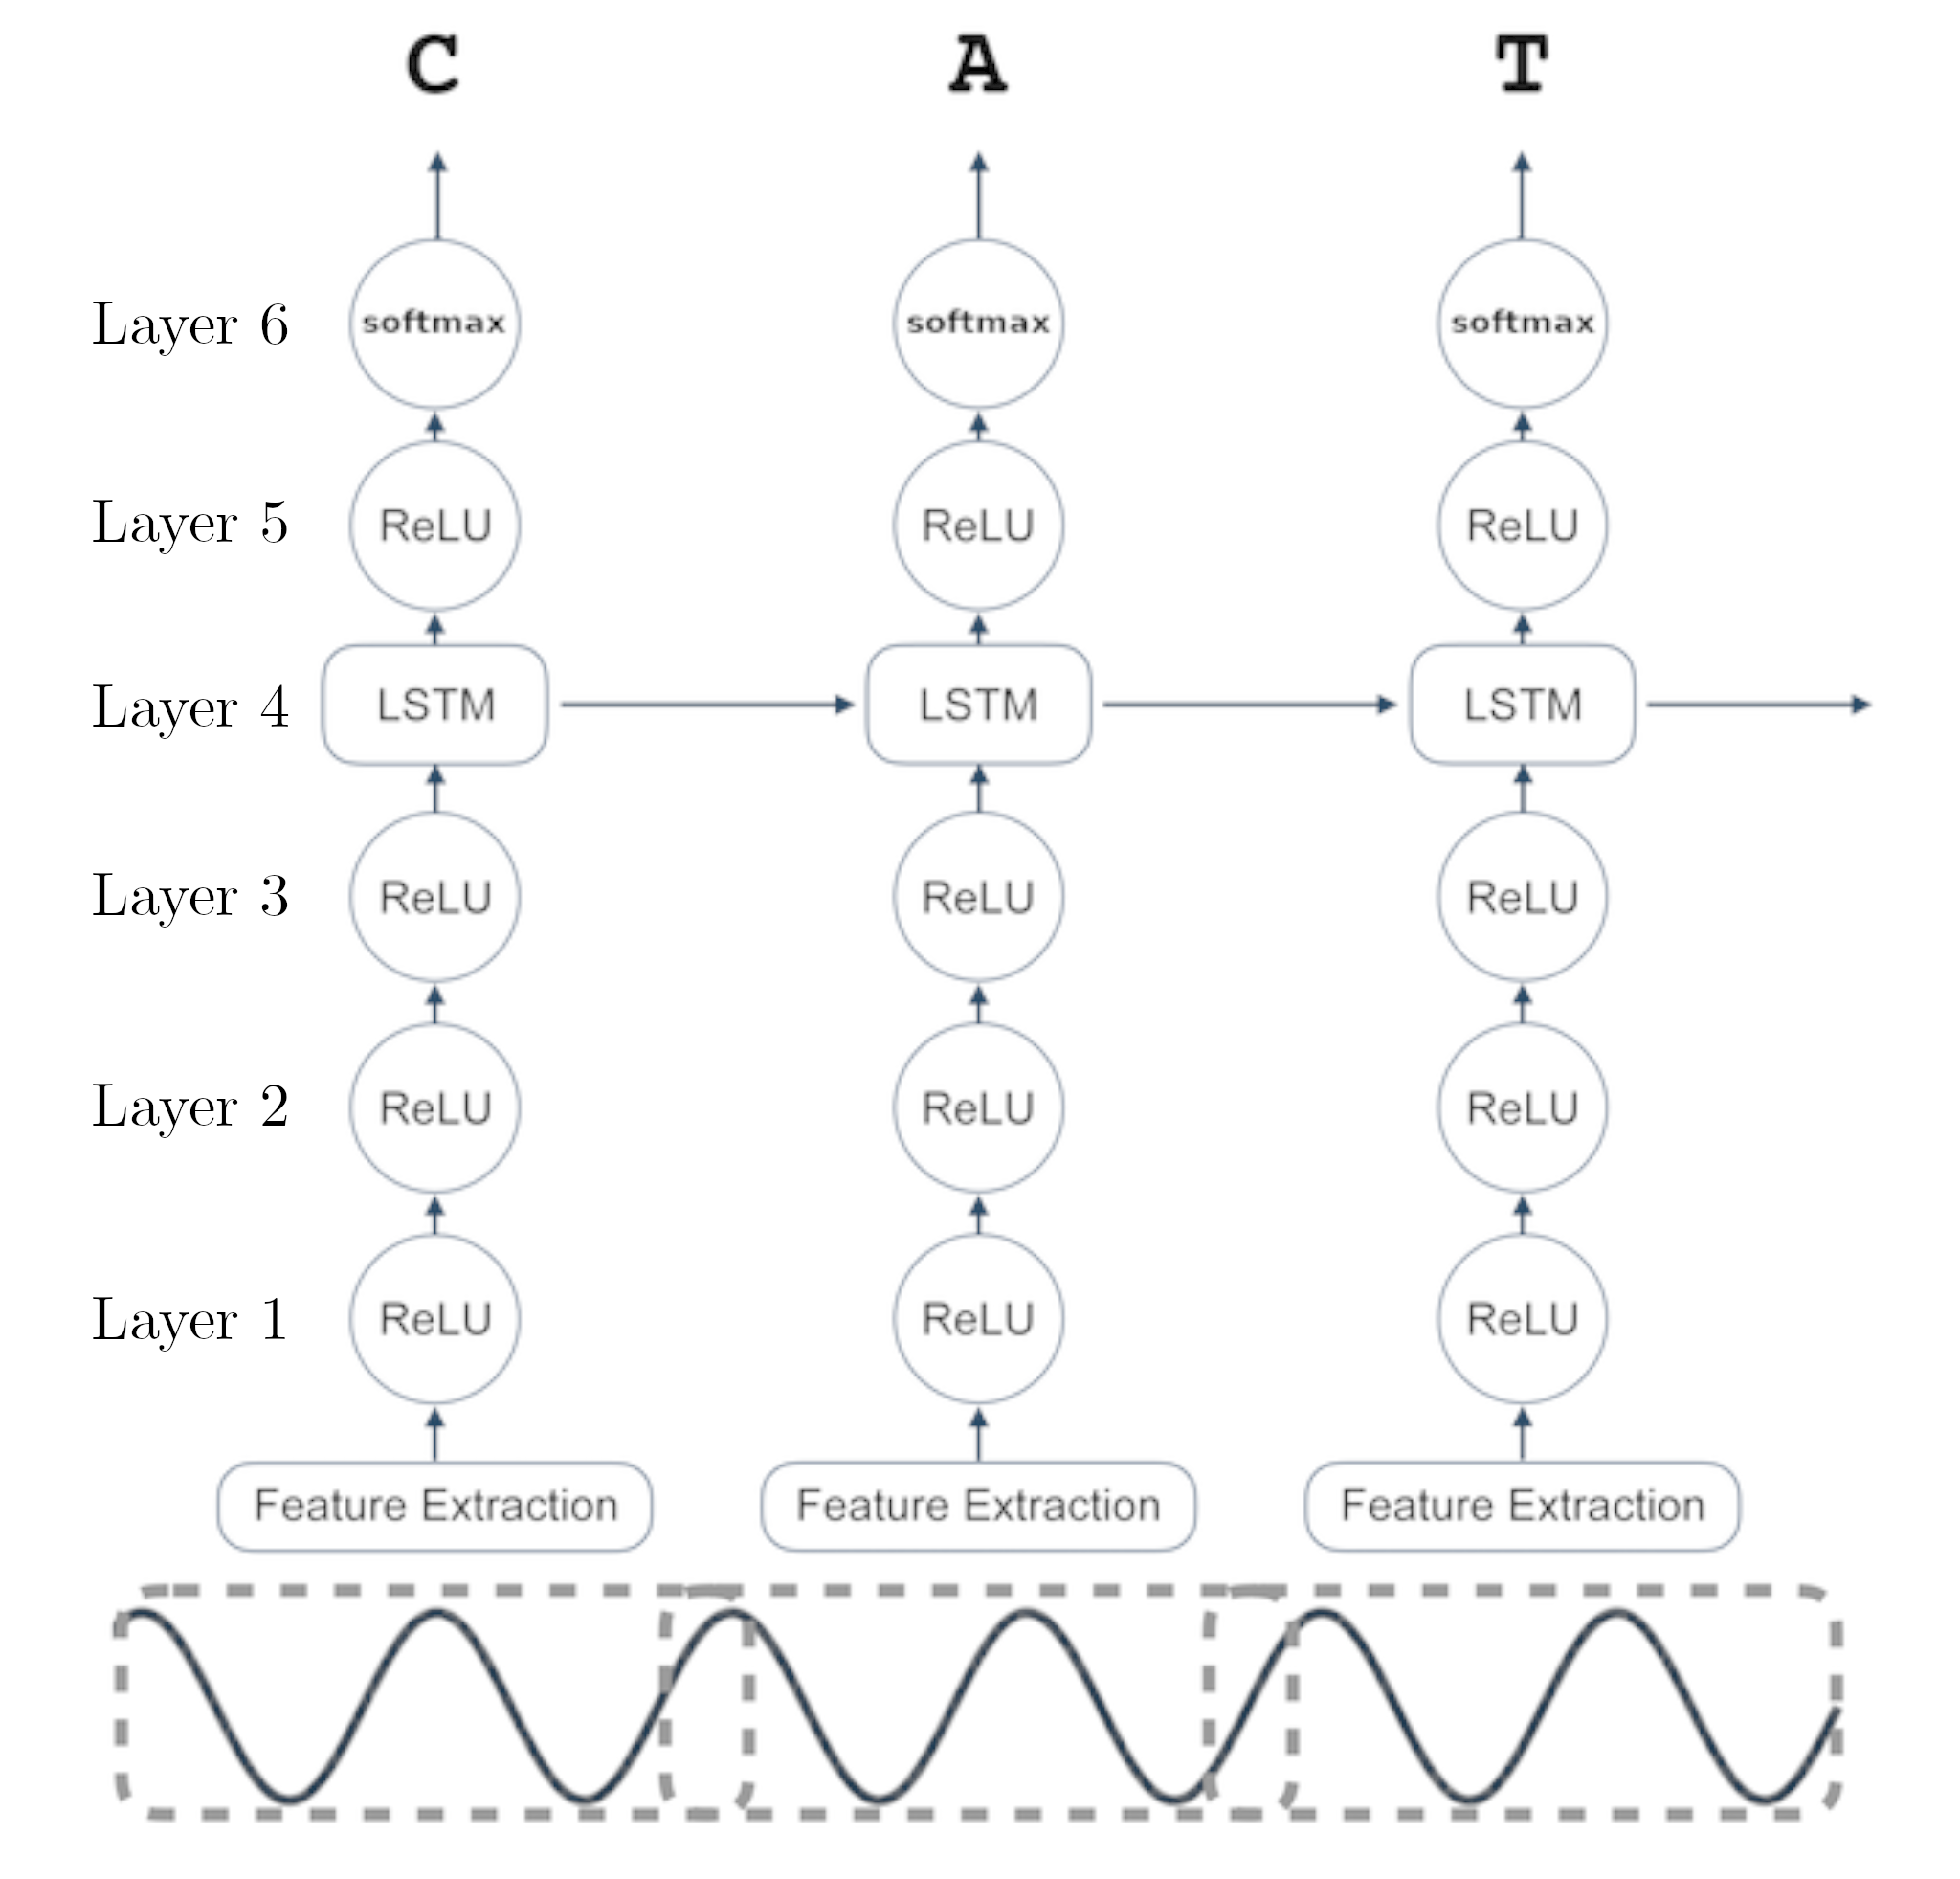
\includegraphics[width=.85\textwidth]{ds.png}
    \caption{DeepSpeech architecture (adapted from the official documentation\protect\footnotemark[\value{footnote}])}
    \label{fig:ds}
\end{figure}

\subsection{Training Details}
% erst: erklären, welche models tatsächlich trainiert wurden. was heißt complete, transfer, etc.
% dann: agarwal, training script, version, implementation and github, dataset, language model, hyperparameters, specs
In transfer learning, all weights of the model are initialized to those of the Enlish pretrained model, which is provided by Mozilla\footnote{\url{https://github.com/mozilla/DeepSpeech/releases}}. In addition to transfer learning, we also train the model from scratch with random weight initialization, thereby reproducing a result from \textcite{agarwal-zesch-2019-german}. In total, we train 6 different models:
\begin{enumerate}
    \item The whole model from scratch ("Complete Training")
    \item The model with weights initialized to those of the English pretrained model ("Simple Transfer")
    \item The English-initialized model with the first layer frozen
    \item The English-initialized model with the first two layers frozen
    \item The English-initialized model with the first three layers frozen
    \item The English-initialized model with the first three and the fifth layer frozen
\end{enumerate}

The layers were frozen by simply adding \texttt{trainable=False} at the appropriate places in the TensorFlow code. For all models, we had to reinitialize the last layer, because of the different alphabet sizes of German and English.

The complete training script is available online\footnote{\url{https://github.com/onnoeberhard/deepspeech-paper/blob/master/training.sh}}. We used Mozilla's DeepSpeech version 0.7.4 for training the model from scratch and version 0.7.3 for the transfer learning approach. The modified versions of DeepSpeech that utilise layer freezing are also available online\footnote{\url{https://github.com/onnoeberhard/deepspeech-transfer}, the different versions with a different number of frozen layers are in the branches \emph{transfer-1}, \emph{\mbox{transfer-2}}, \emph{transfer} and \emph{\mbox{transfer-4}}.}.

We trained the models on the German-language Mozilla Common Voice 2.0 speech dataset\footnote{\url{https://voice.mozilla.org/de/datasets}}. This made it possible to compare our results to \parencite{agarwal-zesch-2019-german}.

For inference and testing we used the language model KenLM \parencite{heafield-2011-kenlm}, fitted to the corpus from \parencite{Radeck-Arneth2015}.

In training each model, we used a batch size of 24, a learning rate of 0.0005 and a dropout rate of 0.4. We did not perform any hyperparamter optimization.

The training was done on a Linux machine with 96 Intel Xeon Platinum 8160 CPUs @ 2.10GHz, 256GB of memory and an NVIDIA GeForce GTX 1080 Ti GPU with 11GB of memory. Each model trained for approximately one hour to get 30 epochs.

\section{Results}
bla bla bla
\begin{table}[ht]
    \centering
    \vspace{5mm}
    \begin{tabular}{lrrr}
        \toprule
        Method & WER \\
        \midrule
        Complete Training & 0.697 \\
        Tranfer: No frozen layers & 0.627 \\
        1 Frozen Layer & 0.483 \\
        2 Frozen Layers & 0.443 \\
        \textbf{3 Frozen Layers} & \textbf{0.437} \\
        4 Frozen Layers & 0.462 \\
        \cite{agarwal-zesch-2019-german} & 0.797 \\
        \bottomrule
    \end{tabular}
    \caption{Quanteneffizienten berechnet mit Gleichung}
    \label{tab:results}
\end{table}

\begin{figure}[ht]
    \centering
    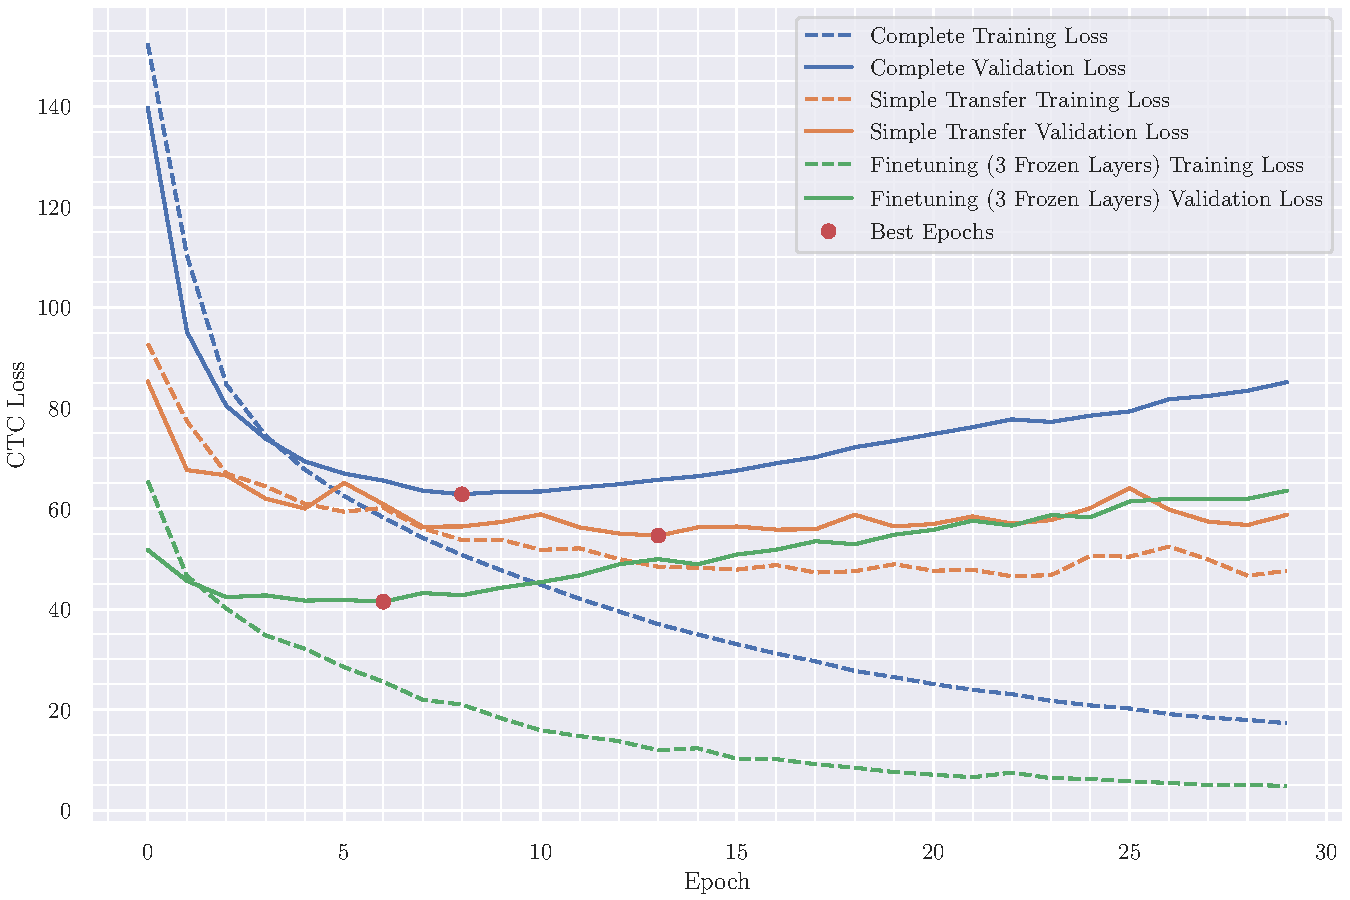
\includegraphics[width=\textwidth]{../3curves.pdf}
    \caption{Trainingskurven..}
    \label{fig:3c}
\end{figure}

\begin{figure}[ht]
    \centering
    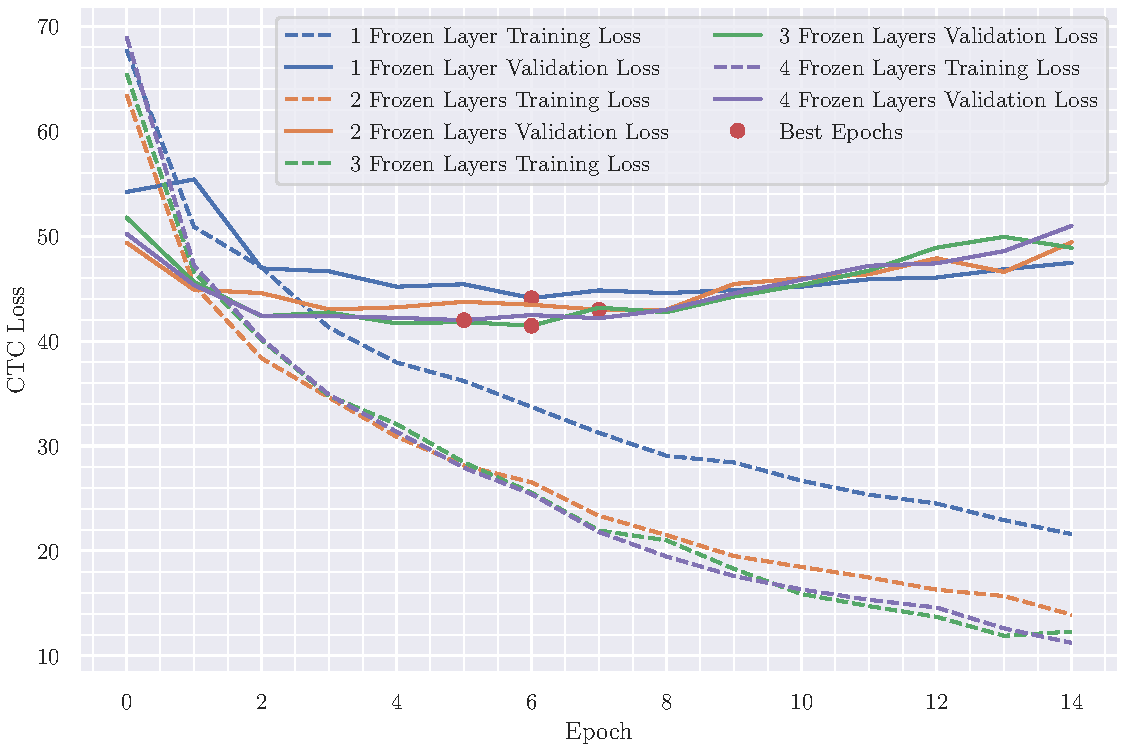
\includegraphics[width=\textwidth]{../4curves.pdf}
    \caption{Trainingskurven 2!..}
    \label{fig:3c}
\end{figure}

\section{Further Research}
% Polyglot
% Training on more data

Citing \cite{agarwal-zesch-2019-german} here.

\printbibliography

\end{document}
